\appendix

\section{Details of Multimodal ArXiv}
\label{apx:arxiv_cap}


\subsection{Caption Cleaning}
\label{apx:caption_clean}

We apply a Python tool to clean the original caption and Table~\ref{tab:pylatexenc_clean} illustrates the caption before and after cleaning. 
\begin{table}[tbh!]
    \centering
    \begin{tabular}{p{3cm}  p{3cm}}
    \toprule
       Before Cleaning & After Cleaning \\
       \midrule
       A 1995 Hale Telescope H$\alpha$ image of the Guitar Nebula (20 angstrom filter at 6564 angstroms). The cometary neck connecting to a spherical bubble are clearly evident. Credit: \textbackslash cite\{cha02\}. &
        A 1995 Hale Telescope H$\alpha$ image of the Guitar Nebula (20 angstrom filter at 6564 angstroms). The cometary neck connecting to a spherical bubble are clearly evident. Credit: \textless cit.\textgreater. \\ 
       \midrule
       As Fig. \textbackslash ref\{z0\} except at $z\sim 6$ ($z=4.37$ in the EdS model). &
    As Fig. \textless ref\textgreater~except at $z\sim 6$ ($z=4.37$ in the EdS model). \\ 
 
       \bottomrule
    \end{tabular}
    \caption{Caption before and after cleaning using pylatexenc.}
    \label{tab:pylatexenc_clean}
\end{table}


\subsection{Illustration Cases of Multimodal ArXiv}
\label{apx:case_illustrations}
We provide illustrated cases from our dataset for a better understanding.
Figure~\ref{fig:single_figure_pair} demonstrates a typical single figure-caption pair, and Figure~\ref{fig:multi_figure_case} shows the multiple figure-caption case.
Figure~\ref{fig:qa_case_1}, \ref{fig:qa_case_2}, \ref{fig:qa_case_3} and \ref{fig:qa_case_4} illustrate the cases from our ArXivQA dataset, covering different figure types and containing diverse questions.



\begin{figure}[htb!]
    \centering
    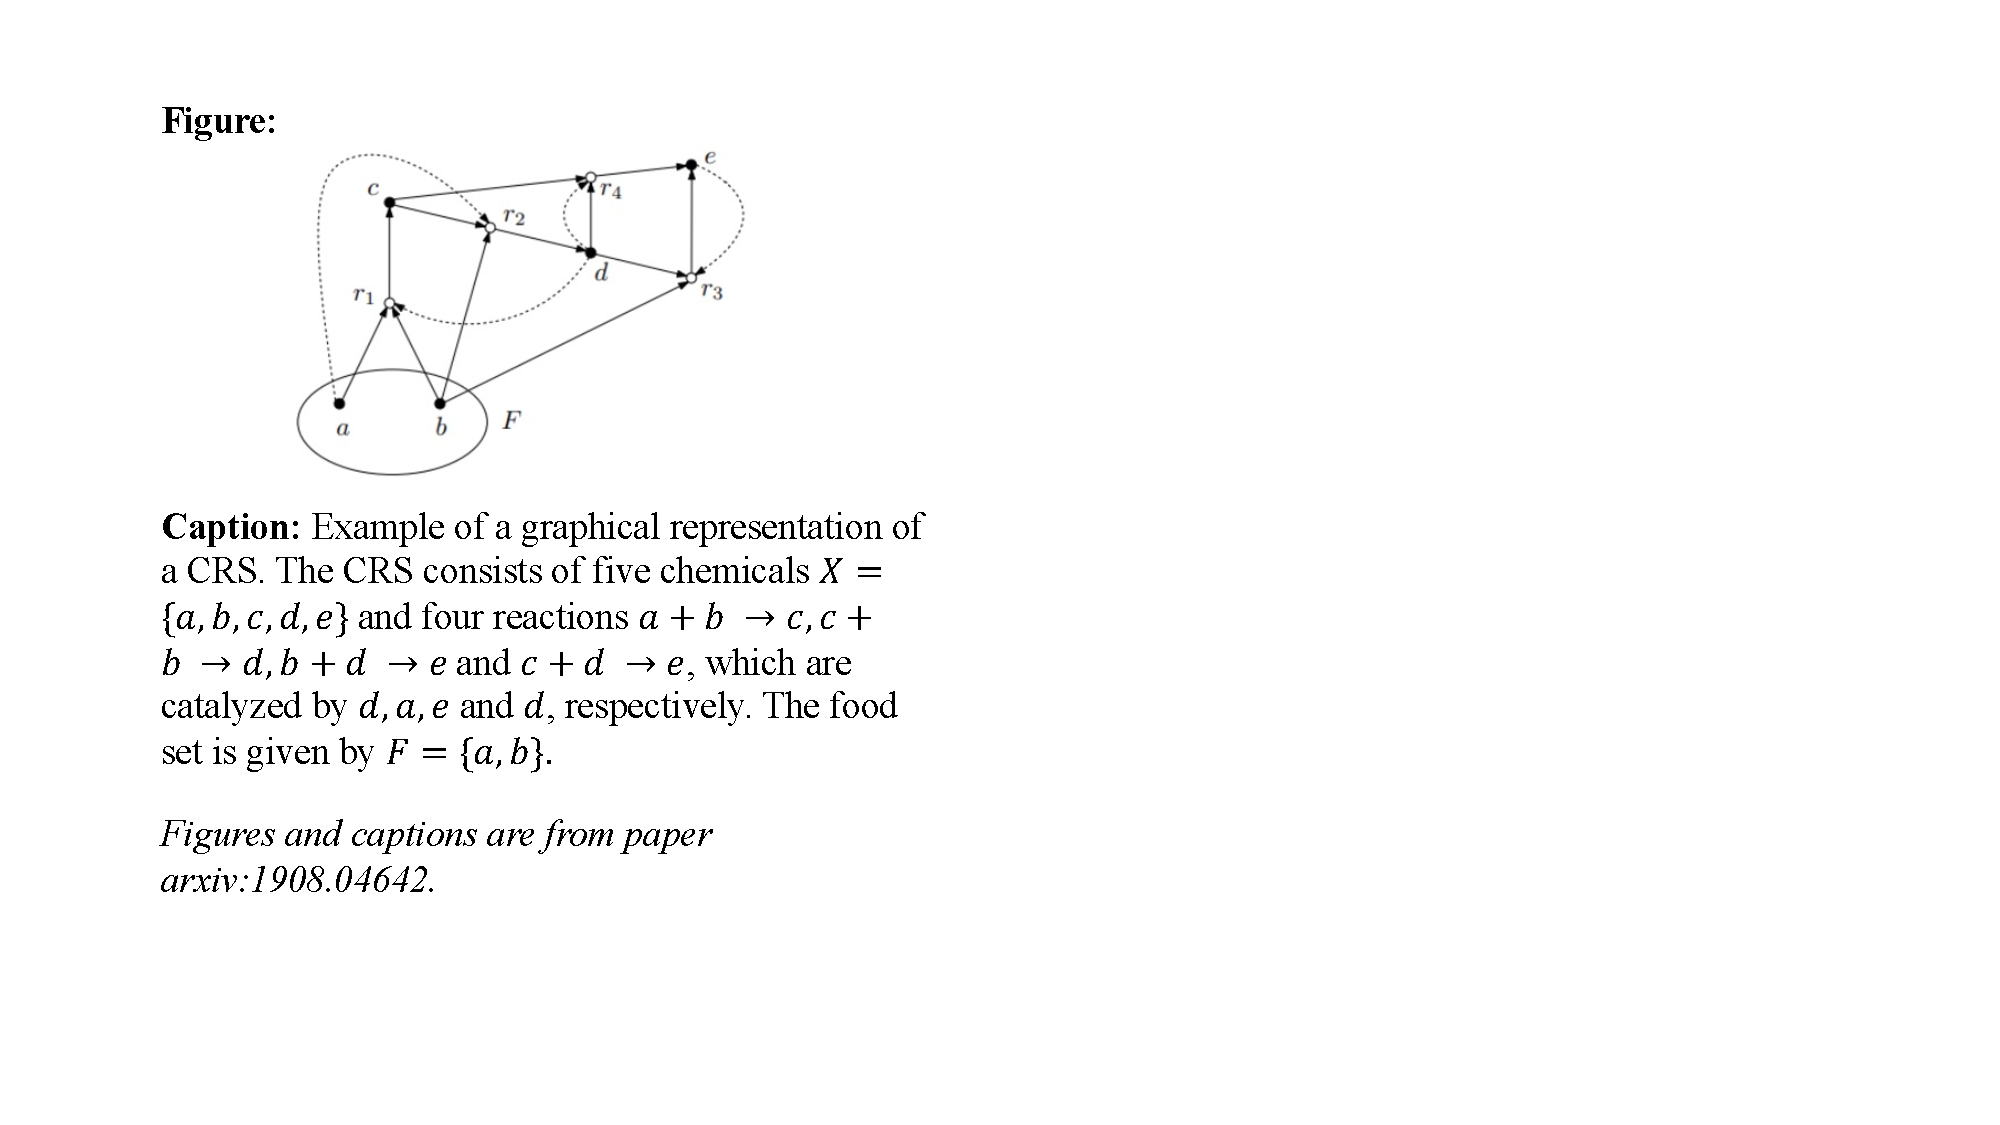
\includegraphics[width=\linewidth]{figs/single-figure-v2.pdf}
    \caption{A single-figure caption pair in our ArXivCap dataset.}
\label{fig:single_figure_pair}
\end{figure}


\begin{figure*}[t!]
    \centering
    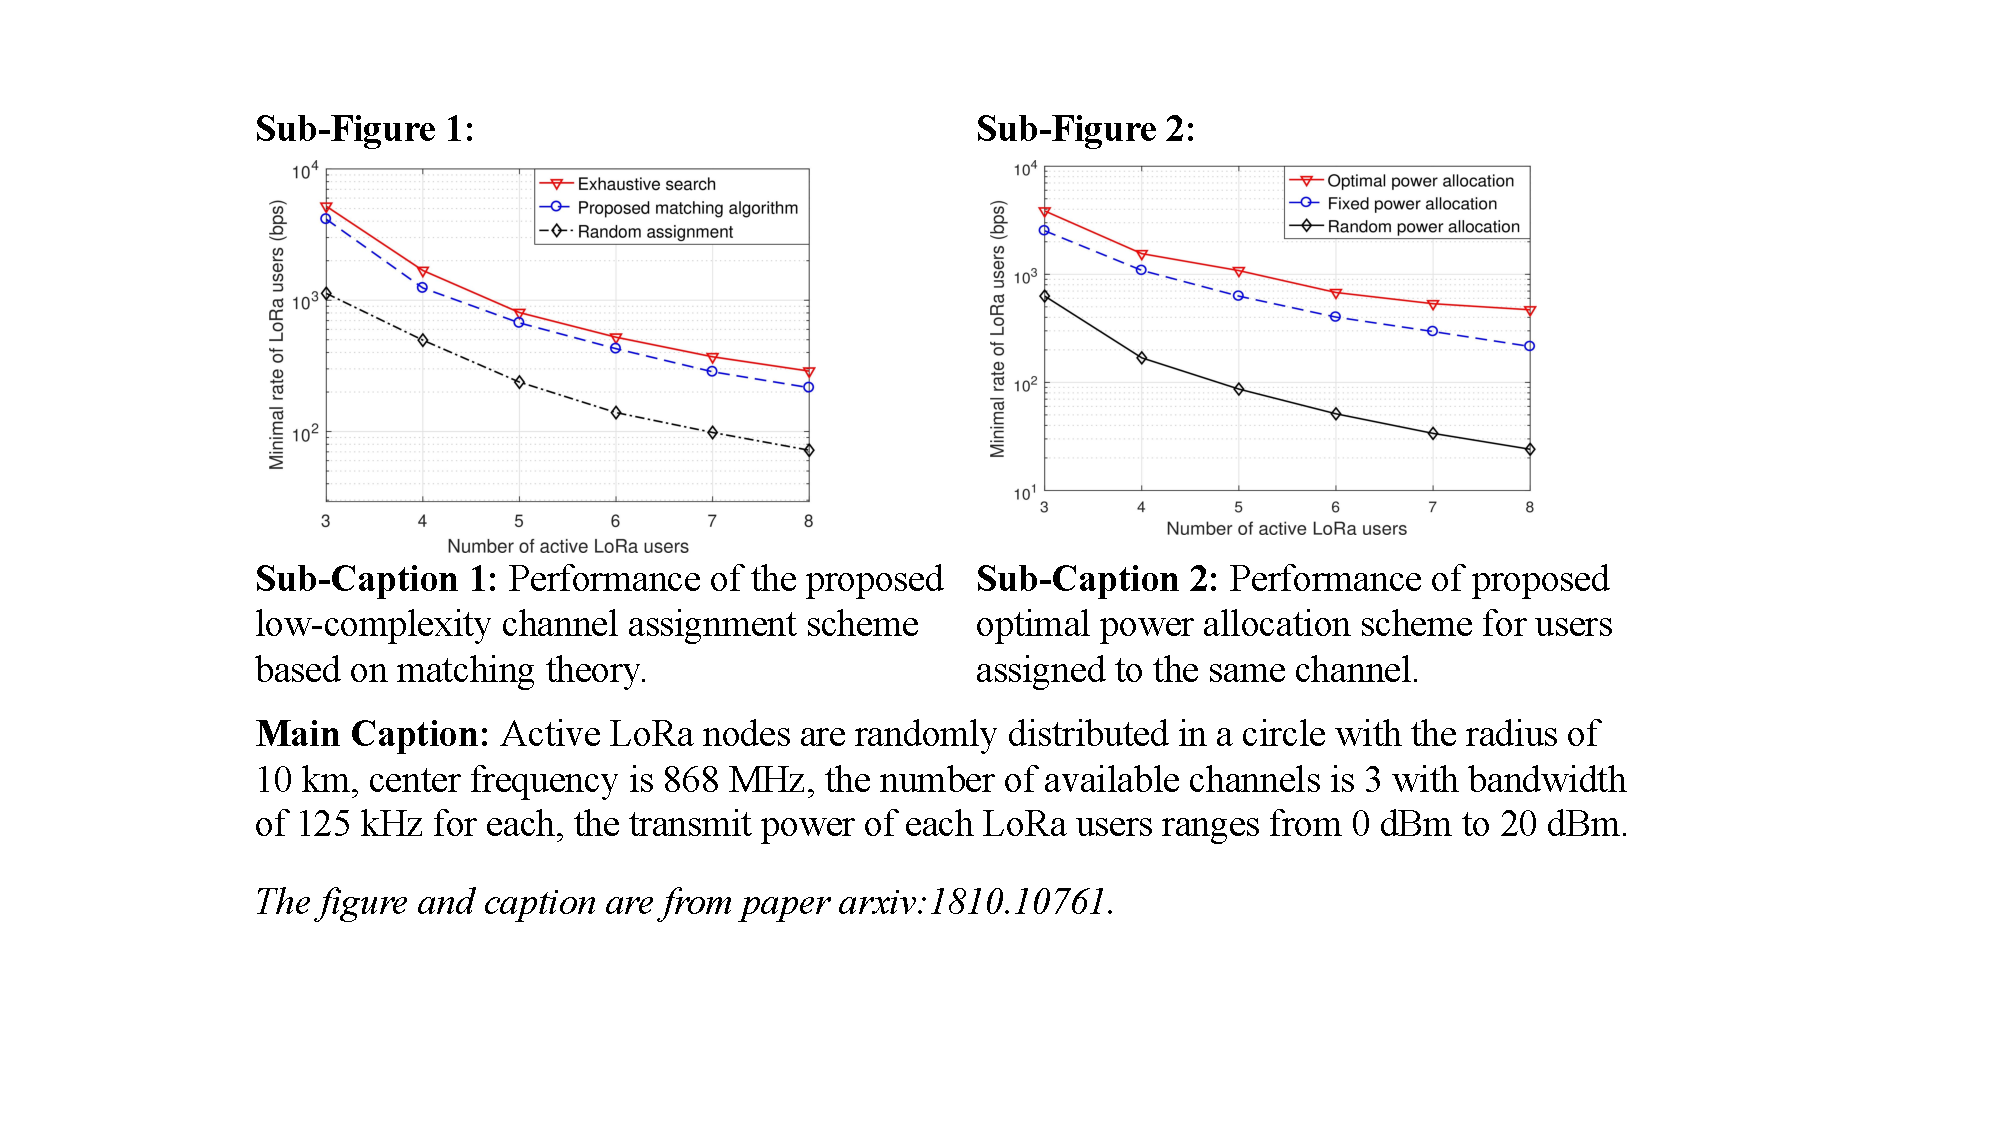
\includegraphics[width=0.85\linewidth]{figs/multiple-figure-v2.pdf}
    \caption{A multiple-figure caption pair in our ArXivCap dataset.}
    \label{fig:multi_figure_case}
\end{figure*}

\subsection{Caption Word Cloud}
\label{apx:caption_word_cloud}

We visualize the word cloud of captions in our ArXivCap dataset in Figure~\ref{fig:word_cloud}. It can be seen that the captions have a diverse vocabulary for describing the different figures in the academic papers.
\begin{figure}[t!]
    \centering
    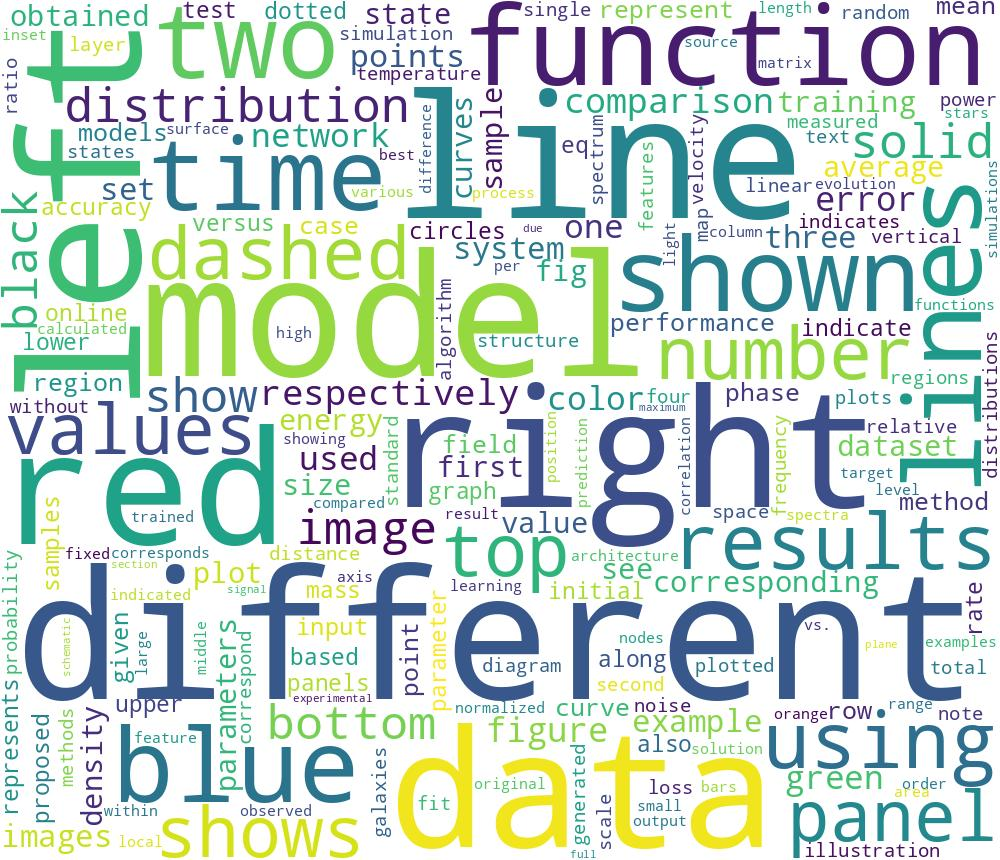
\includegraphics[width=\linewidth]{figs/word_cloud.jpg}
    \caption{Word cloud visualization of captions in our ArXivCap dataset.}
    \label{fig:word_cloud}
\end{figure}




\begin{figure*}[tbh!]
    \centering
    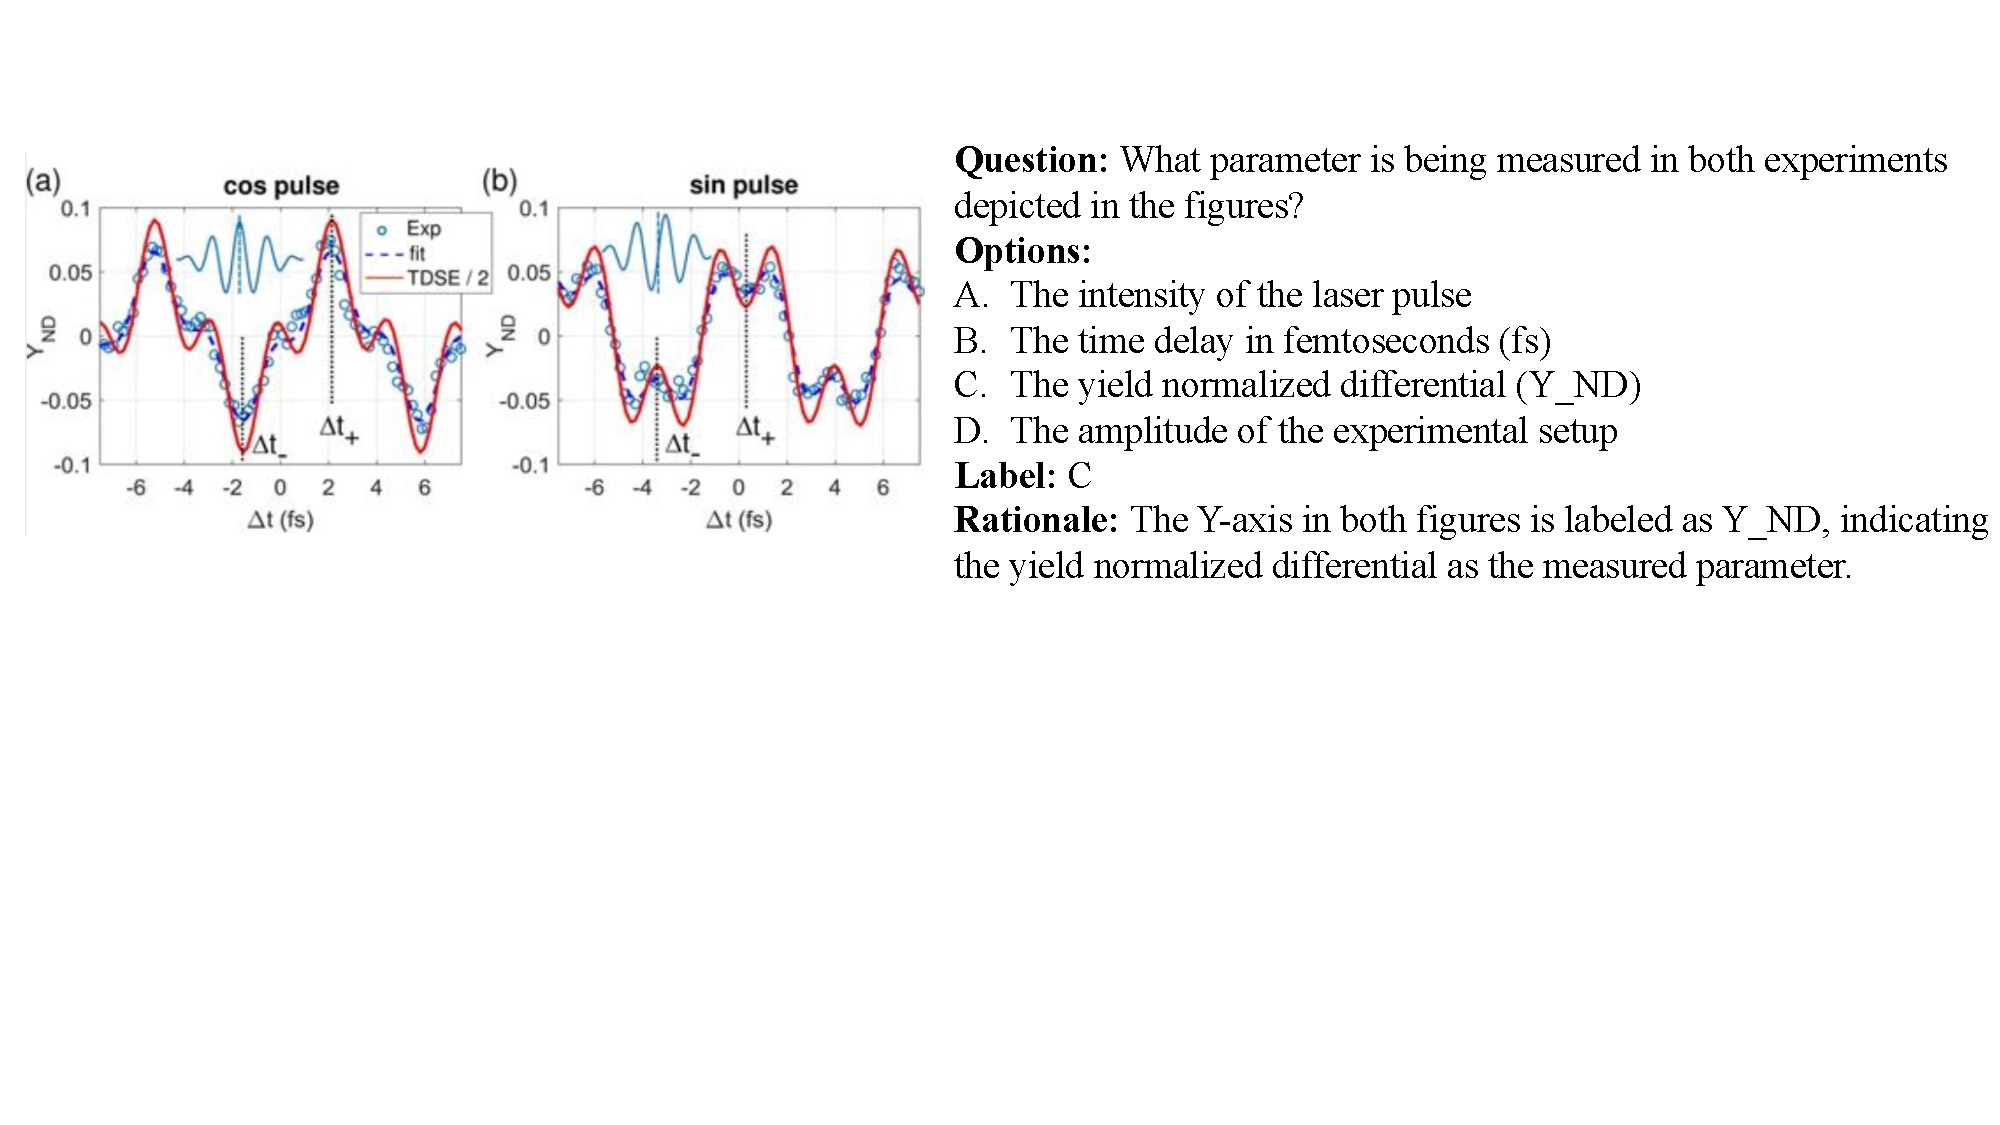
\includegraphics[width=0.85\linewidth]{figs/arxivqa_case1.pdf}
    \caption{A case from our ArXivQA dataset.}
    \label{fig:qa_case_1}
\end{figure*}



\begin{figure*}[tbh!]
    \centering
    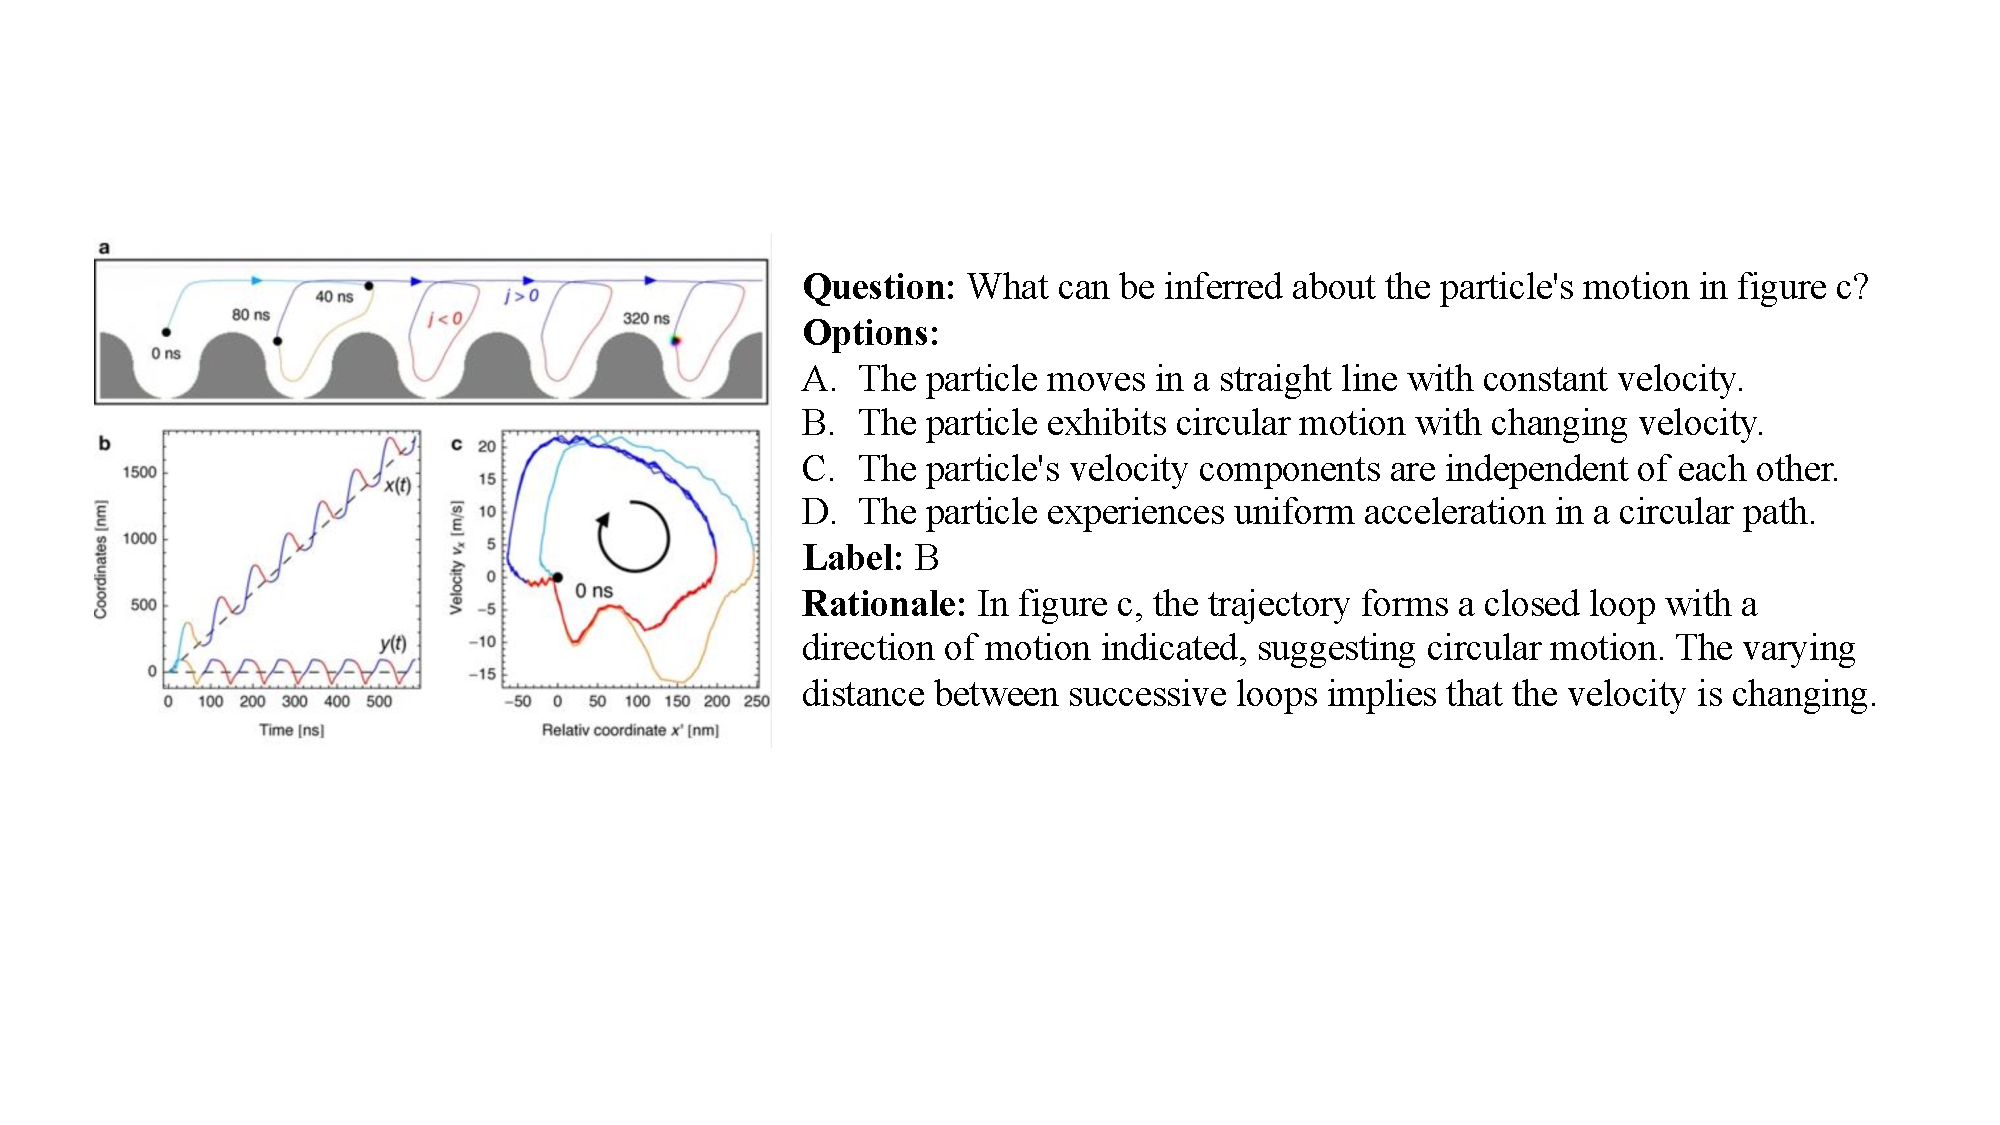
\includegraphics[width=0.85\linewidth]{figs/arxivqa_case2.pdf}
    \caption{A case from our ArXivQA dataset.}
    \label{fig:qa_case_2}
\end{figure*}



\begin{figure*}[tbh!]
    \centering
    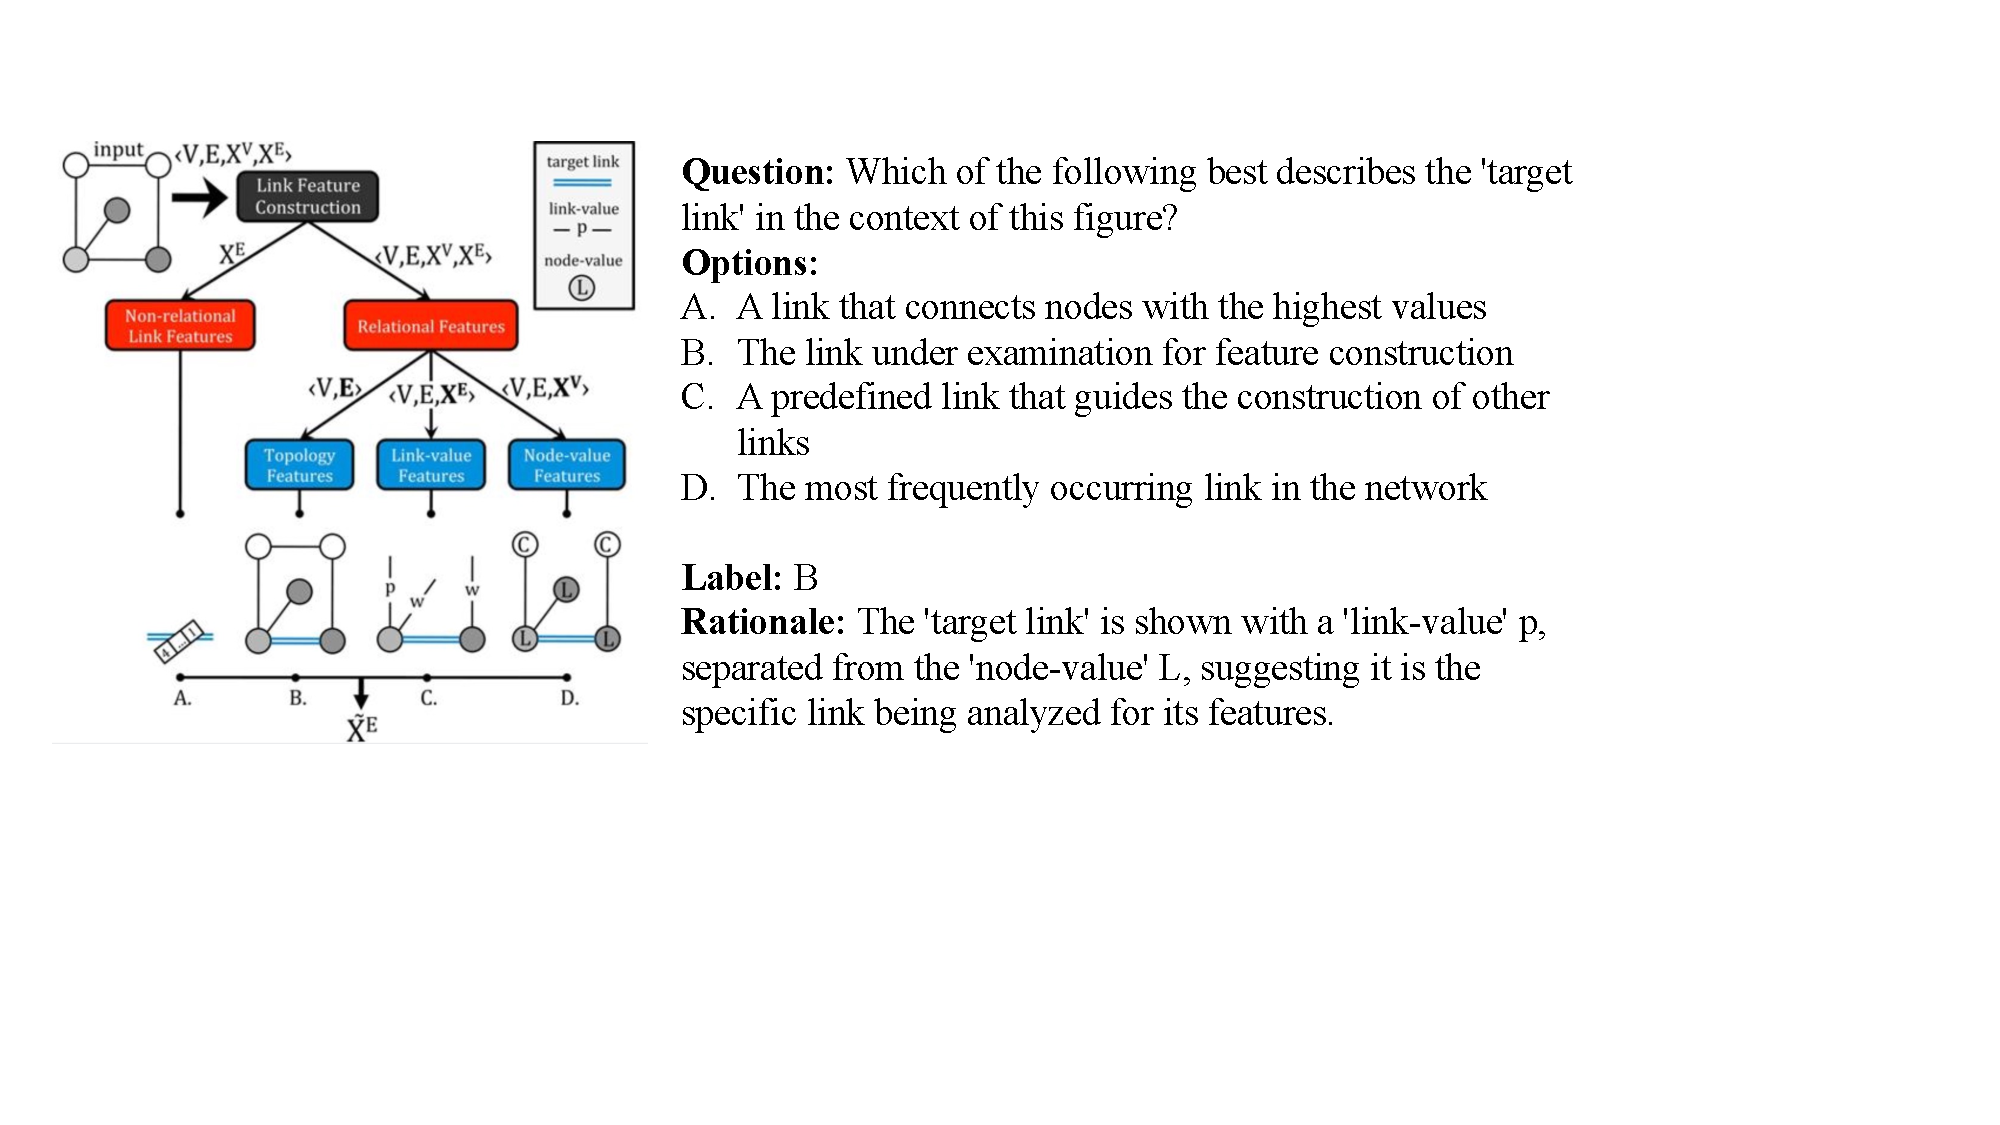
\includegraphics[width=0.85\linewidth]{figs/arxivqa_case3.pdf}
    \caption{A case from our ArXivQA dataset.}
    \label{fig:qa_case_3}
\end{figure*}



\begin{figure*}[tbh!]
    \centering
    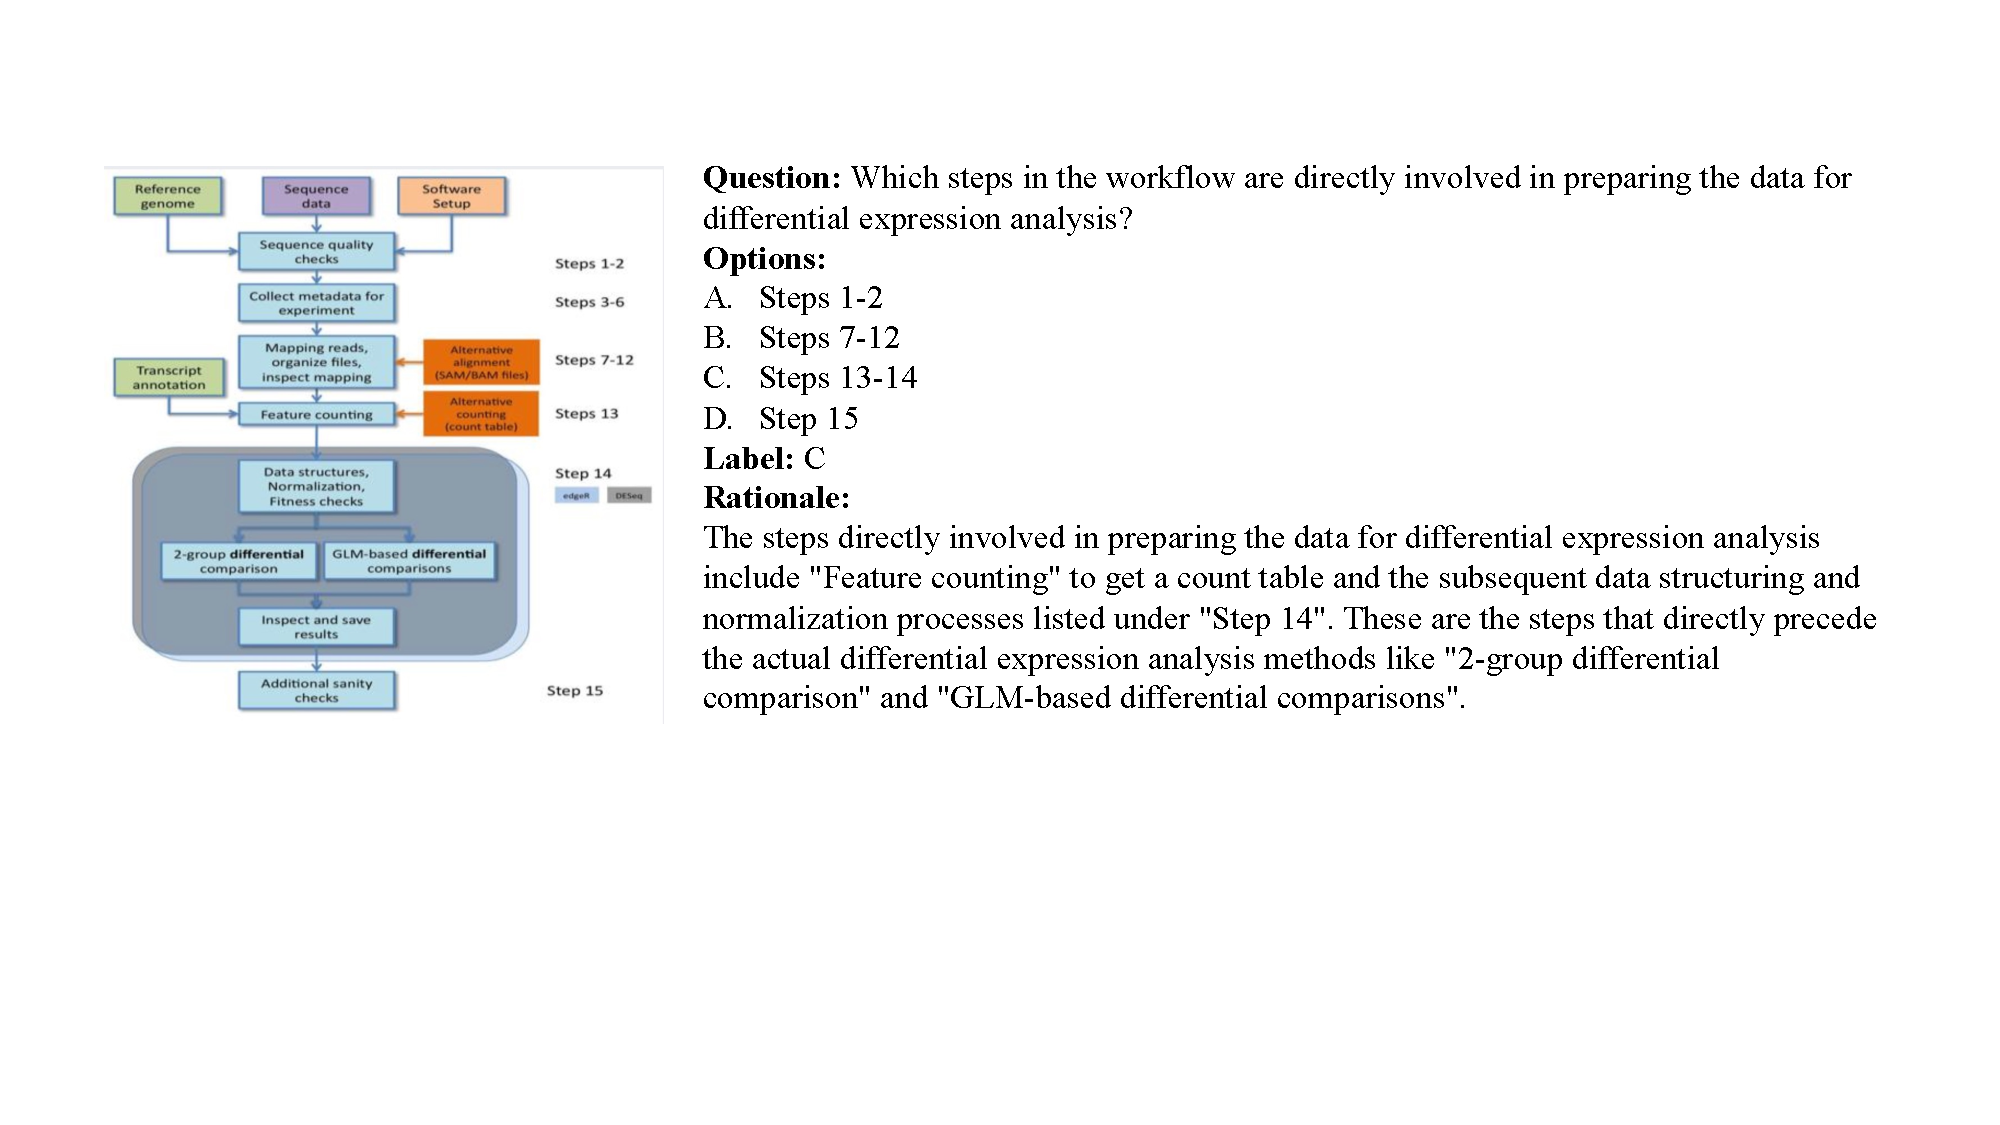
\includegraphics[width=0.85\linewidth]{figs/arxivqa_case4.pdf}
    \caption{A case from our ArXivQA dataset.}
    \label{fig:qa_case_4}
\end{figure*}
\begin{table}[tbh!]
    \centering
    \small 
    \resizebox{\linewidth}{!}{
    \begin{tabular}{l|c}
    \toprule
       Domain  & Full Name \\
       \midrule     
        dg-ga & Differential Geometry \\
        acc-phys & Accelerator Physics  \\
        solv-int & Exactly Solvable and Integrable Systems  \\
        q-alg &  Quantum Algebra and Topology \\
        atom-ph &  Atomic, Molecular and Optical Physics \\
        alg-geom & Algebraic Geometry  \\
        comp-gas &  Cellular Automata and Lattice Gases \\
        supr-con & Superconductivity  \\
        chem-ph &  Chemical Physics \\
        mtrl-th & Materials Theory  \\
        adap-org &  Adaptation, Noise, and Self-Organizing Systems \\
        patt-sol & Pattern Formation and Solitons  \\
        chao-dyn &  Chaotic Dynamics \\
        cmp-lg &  Computation and Language \\
        econ & Economics  \\
        hep-lat & High Energy Physics - Lattice  \\
        nucl-ex & Nuclear Experiment  \\
        q-fin &  Quantitative Finance \\
        math-ph &  Mathematical Physics \\
        nucl-th &  Nuclear Theory \\
        gr-qc & General Relativity and Quantum Cosmology  \\
        hep-ex & High Energy Physics - Experiment  \\
        hep-th & High Energy Physics - Theory \\
        nlin & Nonlinear Sciences \\
        hep-ph & High Energy Physics - Phenomenology \\
        q-bio & Quantitative Biology \\
        quant-ph & Quantum Physics \\
        eess & Electrical Engineering and Systems Science \\
        stat & Statistics \\
        astro-ph & Astrophysics \\
        physics & Physics  \\
        cond-mat & Condensed Matter \\
        math & Mathematics \\
        cs & Computer Science \\
       \bottomrule
    \end{tabular}}
    \caption{Name of each domain.}
    \label{tab:domain-full-name}
\end{table}



\begin{table}[t!]
    \centering
    \tiny 
    \begin{tcolorbox}
Multiple-choice Question Answer Pairs Generation for Scientific Figures

\textbf{Guideline}

The goal of this task is to create answerable multiple-choice questions based on figures from scientific papers, to improve the ability of a large vision language model.

The questions should be challenging, and require college-level reasoning. The type of questions should be diverse. The question should be answerable based on the figure. The answer should be one of the answer choices. The answer choices should be plausible and challenging. 


\textbf{Format}

Below is an example of the format of the input and output for the task.

\textbf{Input}

Figures: [Figures input in the task]

\textbf{Output}

Question: [Question]

Answer Options: [Answer choices, a bullet list.]

Correct Choice: [Correct answer choice, e.g., A]

Rationale: [Rationale for the correct answer, explain why the answer is correct]
    \end{tcolorbox}
    \caption{Prompt used for GPT-4V to generate QA pairs based on scientific figures.}
    \label{tab:prompt_for_ArXivqa}
\end{table}
\subsection{ArXivQA Prompting Template}
\label{apx:prompt_template}
The prompt used to query GPT-4V is provided in Table~\ref{tab:prompt_for_ArXivqa}.

\subsection{Quality Analysis of ArXivQA}
\begin{table*}[t!]
    \centering
    \tiny  
    \begin{tcolorbox}
1. Ensuring Factual Integrity and Clear Presentation:\\
- Factual Alignment: Ensure questions and options are grounded in accurate reflections of the chart data.\\
- Visual Clarity: Maintain high-resolution charts to ensure that all pertinent details are discernible.\\
- Unambiguous Textual Information: Employ precise and unambiguous language to formulate questions and answers, thereby mitigating potential misinterpretations.\\
2. Ensuring Relevance and Integrated Comprehensiveness:\\
- Question and Option Relevance: Charts must align with their questions, and all options should be applicable and relevant to the given data.\\
- Comprehensive Integration: Guarantee the provision of comprehensive information necessary for the interpretation of the chart and the resolution of the question, ensuring a cohesive amalgamation of textual and visual data.\\ 
3. Promoting Fairness and Avoiding Bias:\\
- Equitable Content: Strive for impartiality in the dataset to prevent bias and ensure fair representation of diverse groups and perspectives.\\

Grading Protocol:\\
Each criterion is to be rigorously evaluated for each dataset entry. The assessment is to be conducted on a qualitative scale with three distinct levels: High, Medium, and Low. These levels will denote the degree of conformity to the respective criterion:\\
- 1: High: The dataset entry exhibits exemplary adherence to the evaluation criterion, demonstrating a robust and comprehensive alignment with the specified standard.\\
- 0.5: Medium: The dataset entry meets the evaluation criterion to a moderate extent, indicating a satisfactory but not optimal congruence with the standard.\\
- 0 Low: The dataset entry falls short of the evaluation criterion, signaling a need for significant improvements to meet the standard.
    \end{tcolorbox}
    \caption{Annotator guideline of ArXivQA manual quality examination.}
    \label{tab:quality_analysis_ArXivqa}
\end{table*}

\begin{table}[t!]
    \centering
    \small 
    \begin{tabular}{@{}lc@{}}
         \toprule
         Aspect & Avg Score \\
         \midrule
        Factual Alignment & 0.6975 \\
        Visual Clarity & 0.9925 \\
        Unambiguous Textual Information & 0.9825 \\
        Question and Option Relevance & 0.9375 \\
        Comprehensive Integration & 0.905 \\
        Equitable Content & 1.0 \\
        \midrule
        Score Sum & 5.515 \\
        \bottomrule
    \end{tabular}
    \caption{Manual quality analysis of ArXivQA. The average scores for each aspect are presented.}
    \label{tab:quality_analysis_ArXivqa_result}
\end{table}
To evaluate the quality of ArXivQA, we manually assess it from six different aspects. We develop a quality examination guideline for annotators, as shown in Table~\ref{tab:quality_analysis_ArXivqa}, which addresses various aspects of the QA pairs.
We sample 100 examples and ask four authors to conduct the quality analysis. The four authors are divided into two groups, with each group tasks with evaluating 50 examples across six sub-aspects, according to the grading protocol. 

The evaluation results are presented in Table~\ref{tab:quality_analysis_ArXivqa_result}.
We find that most samples feature clear, high-quality images with clear and high-quality images, with unambiguous question and option descriptions. However, a small fraction of the generated questions may be unanswerable due to mis-recognizing elements in the figures, as reflected by lower factual alignment scores. Additionally, we consider samples with an aggregate score of 5 or higher from both annotators to be of sufficient quality. Under this stringent criterion, 79 out of 100 samples meet the threshold, demonstrating that the dataset's quality is generally satisfactory.

\section{Evaluation Details}
\label{apx:evaluation_details}
\subsection{Details of Evaluated Models}


\paragraph{BLIP2}~\citep{li2023blip2}, 
introduces a lightweight Q-Former designed to bridge modality gaps and leverages frozen LLMs. Leveraging LLMs, BLIP-2 can conduct zero-shot image-to-text generation using natural language prompts. We select the \texttt{BLIP2-OPT-6.7B} version for evaluation.\footnote{\url{https://huggingface.co/Salesforce/blip2-opt-6.7b}}


\paragraph{InstructBLIP}~\citep{dai2023instructblip} employs an instruction-aware visual feature extraction module based on BLIP2~\citep{li2023blip2} and is trained with unified multimodal instruction tuning datasets. We choose \texttt{InstructBLIP-Vicuna-7B} for evaluation.\footnote{\url{https://huggingface.co/Salesforce/instructblip-vicuna-7b}}.



\paragraph{LLaVA}~\citep{liu2023llava},
adopts Vicuna models as the backbone LLM and is trained on the ChatGPT/GPT-4 generated instruction tuning dataset.
LLaVA-v1.5~\citep{liu2023llava15} improves on LLaVA models by employing curated task datasets and an enhanced modality alignment module.
We evaluate both \texttt{LLaVA-v1.5-7B}\footnote{\url{https://huggingface.co/liuhaotian/llava-v1.5-7b}} and \texttt{LLaVA-v1.5-13B}.\footnote{\url{https://huggingface.co/liuhaotian/llava-v1.5-13b}}


\paragraph{Flamingo}~\citep{Alayrac2022FlamingoAV} pioneers the development of LVLMs by introducing a cross-gated layer for LLMs to produce visual-grounded text. The training dataset
consists of interleaved visual data and text from the web pages, enabling it to generate free-form text as the output. We select the open-source implementation \texttt{OpenFlamingo-9B}~\citep{awadalla2023openflamingo} for evaluation.\footnote{\url{https://huggingface.co/openflamingo/OpenFlamingo-9B-vitl-mpt7b}}

\begin{table*}[t!]
    \centering
\tiny 
\begin{tcolorbox}
Annotation Instruction:\\
As an annotator, your role is to serve as an unbiased and objective judge in evaluating the accuracy of captions produced by a Large Vision-Language Model (LVLM) for scientific figures. These figures are extracted from academic papers, and to aid your assessment, we will provide you with the paper's title and abstract for necessary context.

You will be presented with the original caption—referred to as the 'ground truth'—and the LVLM generated caption, termed the 'prediction'. You could take into account the context given by the paper's title and abstract for background knowledge, comparing it critically with both captions.

In your assessment, please pay attention to the factual alignment, including but not limiting to the following aspects:\\
- Numerical data and statistics: Verify their accuracy and correspondence to the data presented in the figure.\\
- Symbols: Check for correct representation and usage in the context of the scientific subject matter.\\
- Factual content: Ensure all facts are consistent with those stated in the ground truth caption and the paper's content.\\

<title>{title}</title>\\
<abstract>{abstract}</abstract>\\
<ground truth>{gt}</ground truth>\\
<prediction>{pred}</prediction>\\

Compare the prediction to the ground truth, provide a brief analysis, and assign a score using one of the following quality labels: <Perfect>, <Good>, <Fair>, <Poor>, <Incorrect>.

Below we describe the detail criteria for score:
<Perfect>: The prediction is almost identical to the ground truth, with only minor, inconsequential differences that do not change the meaning. All numerical data, symbols, and factual content are accurate and consistent.\\
<Good>: The prediction is largely similar to the ground truth but has some noticeable differences that may slightly change the meaning. However, the core information is still correct, and the numerical data, symbols, and factual content are mostly accurate and consistent with the figure content.\\
<Fair>: The prediction captures the basic idea of the ground truth but has significant differences that change the meaning in a way that cannot be ignored. There may be some inaccuracies or inconsistencies in the numerical data, symbols, or factual content when compared to the figure content.\\
<Poor>: The prediction is related to the ground truth but has serious errors or omissions that significantly change the meaning. The numerical data, symbols, or factual content may be largely inaccurate or inconsistent with the figure content.\\
<Incorrect>: The prediction is completely different or irrelevant to the ground truth, with no similarities between the two. The numerical data, symbols, and factual content are entirely inaccurate or inconsistent with the figure content.

Give a brief analysis within 100 words and then output a quality label wrapped with "<>".
    \end{tcolorbox}
    \caption{Prompt template designed for GPT-4 to evaluate generated captions based on the paper title, abstract, and ground truth.}
    \label{tab:prompt_for_gpt4_score_caption}
\end{table*}

\begin{table}[t!]
    \centering
    \small  
    \resizebox{\linewidth}{!}{
    \begin{tabular}{@{}lcccc@{}}
         \toprule
         Model & BLEU-2 & ROUGE-L & BERT-S & GPT-4 Score \\
         \midrule
BLIP-2-OPT-6.7B & 1.5 & 6.6 & 81.3 & 1.18 \\
InstructBLIP-Vicuna7B & 3.5 & 10.3 & 83.6 & 1.48 \\
LLaVA-1.5-7B & 2.3 & 10.4 & 83.3 & 1.80 \\
LLaVA-1.5-13B & 2.7 & 11.0 & 83.6 & 1.69 \\
OpenFlamingo-9B & 5.8 & 10.3 & 82.7 & 1.52 \\
IDEFICS-Instruct-9B & 2.1 & 9.3 & 83.8 & 1.55 \\
Qwen-VL-Chat & 4.7 & 11.1 & 82.0 & 1.81 \\
Qwen-VL-Chat tuned w/ ArXivCap & 8.6 & 15.3 & 83.2 & 2.03 \\
         \bottomrule
    \end{tabular}}
    \caption{Results of 500 single-figure captions generated by various models.}
    \label{tab:gpt4_score_single_caption}
\end{table}



\paragraph{IDEFICS} is another open-sourced implementation of Flamingo~\citep{Alayrac2022FlamingoAV}. Trained on publicly available image-text alignment pairs and instruction tuning datasets, it demonstrates comparable results with the original closed-source model on various image-text benchmarks. We select the \texttt{IDEFICS-Instruct-9B} for evaluation.\footnote{\url{https://huggingface.co/HuggingFaceM4/idefics-9b-instruct}}.

\paragraph{Qwen-VL-Chat}~\citep{Qwen-VL} is
a bilingual LVLM that supports both English and Chinese built on the Qwen LLM~\citep{qwen}. 
During the training phase, Qwen-VL-Chat adopts a packing strategy to create multiple images as inputs,
improving its ability to understand the vision context. We select the \texttt{Qwen-VL-Chat-7B} for evaluation.\footnote{\url{https://github.com/QwenLM/Qwen-VL}}



\paragraph{GPT-4V}
~\citep{gpt4v}, the proprietary vision-language models developed by OpenAI, which are shown to be powerful on various multi-modal tasks~\citep{yang2023dawn}. The API version we queried is \texttt{gpt-4-vision-preview}.

\paragraph{Bard}~\citep{bard}, a commercial LVLM developed by Google. We utilize the unofficial API\footnote{\url{https://github.com/dsdanielpark/Bard-API}} querying the model with our task prompts, accessed on \texttt{2023-11-17}.

\paragraph{Gemini 1.0 Pro Vision}~\citep{reid2024gemini}, a upgraded LVLM by Google. We utilize the official API querying the model with our task prompts, accessed on \texttt{2024-05-20}.


\subsection{Task Prompts}
We evaluate all the models with the same task prompts in our experiments, and the prompts for our four tasks are listed below:

\noindent\textbf{Single-Figure Captioning}:  \texttt{Create a caption for the provided figure.}

\noindent\textbf{Multiple-Figure Captioning} \texttt{Create a caption for the provided figures.}

\noindent\textbf{Contextualized Captioning}: We reuse the prompts in previous captioning tasks depending on the current figure type.

\noindent\textbf{Title Generation}: \texttt{
According to the figures and captions, generate a title for this paper. Title:} 


\subsection{GPT-4 Evaluation of Caption}
\label{apx:gpt4_eval}


In addition to BLEU-2, ROUGE-L, and BERT-S, we also utilize GPT-4 to evaluate a sample of 500 generated captions. Specifically, we employ GPT-4 for the evaluation of single-figure caption tasks following FairEval~\citep{wang2023large}.
The template for prompting GPT-4 to evaluate generated captions is presented in Table~\ref{tab:prompt_for_gpt4_score_caption}. GPT-4 is asked to perform an analysis and then produces a quality score, which is subsequently mapped to a scale from 1 to 5.
The results are presented in Table~\ref{tab:gpt4_score_single_caption}. We observe that the ROUGE-L metric exhibits the highest correlation with the GPT-4 Score (Pearson r = 0.91), followed by BLEU-2 (Pearson r = 0.64). BERT-S instead demonstrates a moderate correlation (Pearson r = 0.39).
The uniformly low GPT-4 scores across all models suggest that they struggle to produce satisfactory captions, which is consistent with the findings in our main paper. Notably, training on ArXivCap results in a significant 12\% improvement in the GPT-4 score compared to the original Qwen-VL-Chat model, leading to the most favorable outcomes in this evaluation.

\section{Error Analysis}
\label{apx:case}
\begin{figure*}[t!]
    \centering
    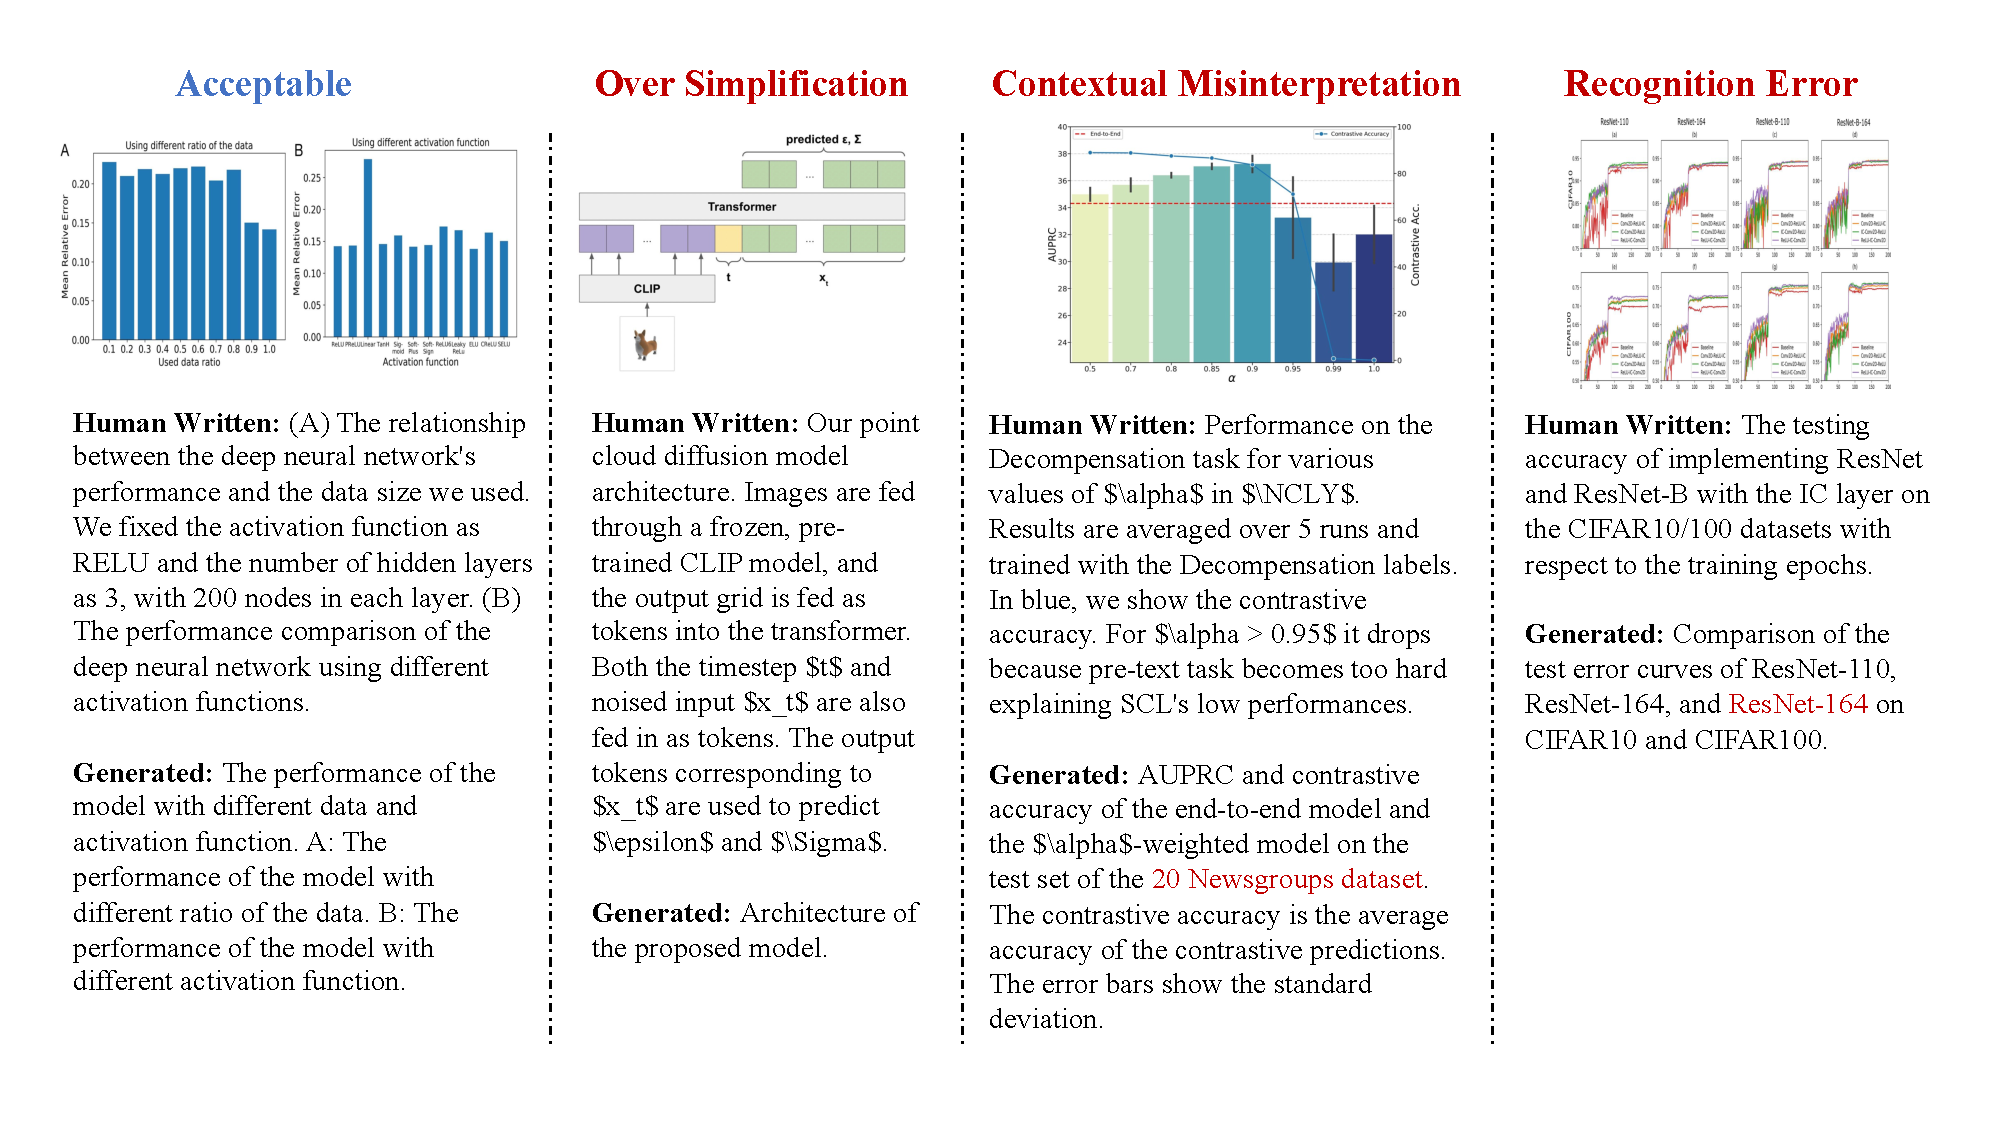
\includegraphics[width=0.95\linewidth]{figs/caption_error_type.pdf}
    \caption{Illustration of acceptable and three error types of generated captions.}
    \label{fig:caption_type}
\end{figure*}


\begin{figure}[t!]
    \centering
    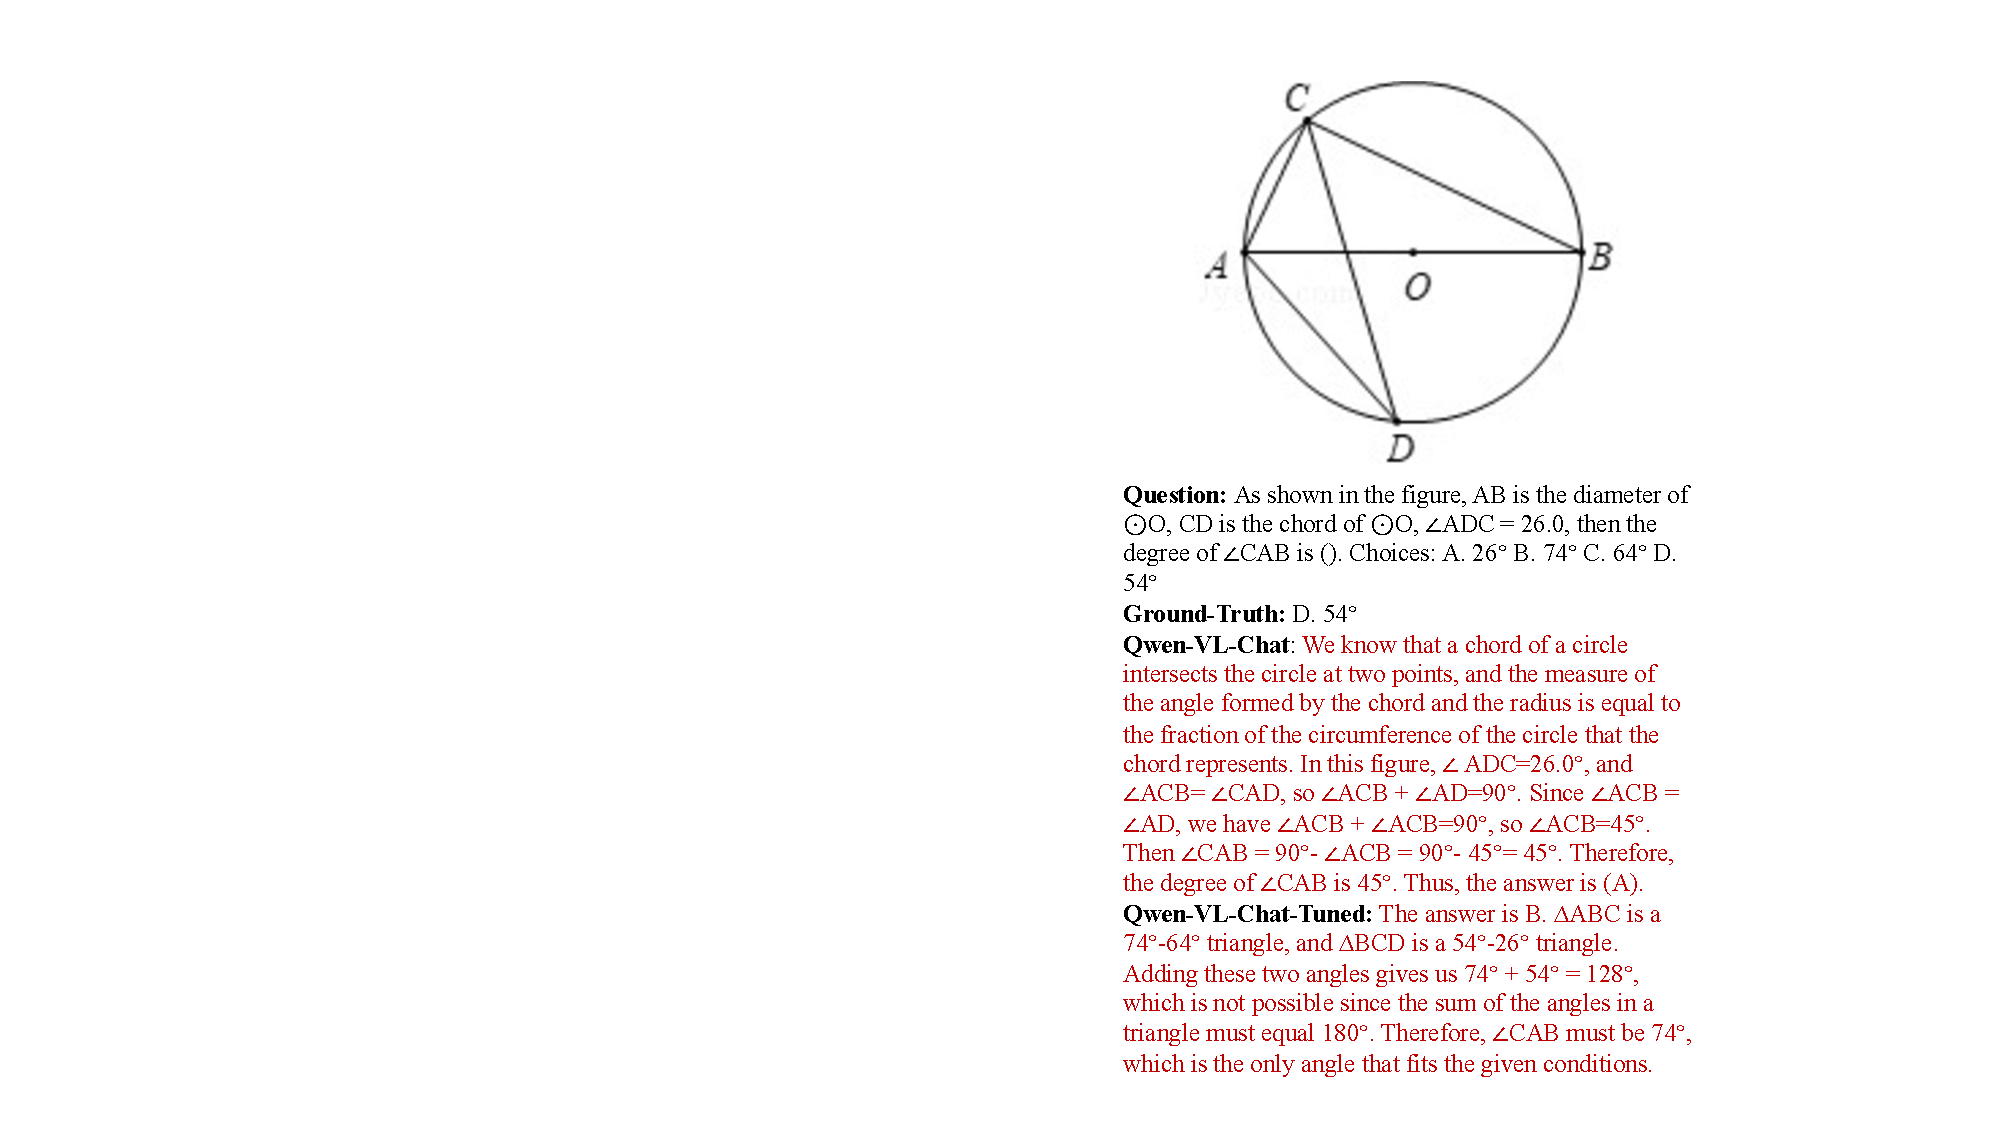
\includegraphics[width=0.85\linewidth]{figs/mathvista_both_wrong.pdf}
    \caption{A failure case on the geometry problem-solving task.}
\label{fig:geometry_fail}
\end{figure}
\subsection{Caption Type Illustration} 
\label{apx:caption_type}
We illustrate captions of four types in our main paper in Figure~\ref{fig:caption_type}. The \emph{Acceptable} caption provides a comprehensive description of the figure presented. The \emph{oversimplified} caption is too short compared with the original human-written caption. 
Furthermore, as shown in the third block in Figure~\ref{fig:caption_type}, \emph{Contextual Misinterpretation} refers to captions with unmentioned content in the figure, such as the dataset colored in red.
\emph{Recognition Error} denotes the model wrongly identified the number or text in the figure, such as the misidentified model name in the last block of Figure~\ref{fig:caption_type}.

\subsection{Failure Sample of MathVista}
\label{apx:failure_mathvista}
Figure~\ref{fig:geometry_fail} shows a challenging geometry mathematic reasoning problem where both models fail to produce the correct answer.
Echoing the quantitative results in our main paper, we believe future studies can incorporate more focused corpus for enhancing the geometry and mathematical reasoning ability of LVLMs.

\section{Results with LLaVA Backbone}
\label{apx:llava}

\begin{table*}[t!]
    \centering
    \small 
    \begin{tabular}{l|c c c c}
        \toprule
        Model & MathVista & MMMU(val) & ScienceQA(IMG only) & MM-Vet \\
        \midrule
        LLaVA-v1.5-7B & 26.6 & 35.3 & 66.8 & 30.5 \\
        \quad Original SFT +ArXivQA & \textbf{28.2} & \textbf{36.0} & \textbf{68.3} & \textbf{32.4} \\
        \bottomrule
    \end{tabular}
    \caption{After fine-tuning with a combination of ArXivQA and original SFT data, the LLaVA model shows boosted mathematical reasoning abilities across benchmarks.}
    \label{tab:llava_performance}
\end{table*}

We investigate whether ArXivQA could also enhance other LVLMs, such as LLaVA models~\citep{liu2023llava}. To maintain model performance, we mix our ArXivQA dataset with the LLaVA SFT 665K-instruction tuning dataset. The LLaVA-v1.5-7B is adopted as the backbone and the model is trained following the original recipe. The results on various benchmarks are listed in Table \ref{tab:llava_performance}.
We find that not only the scientific reasoning performance is improved on multimodal reasoning tasks (MathVista \citep{mathvista}, MMMU \citep{mmmu}, and ScienceQA \citep{lu2022scienceqa}), but the overall capability on MM-Vet \citep{yu2024mmvet} is also boosted. Together with our results using Qwen-VL-Chat, these findings indicate that our ArXivQA dataset can enhance different model backbones and is beneficial across various benchmarks.